\documentclass[11pt]{article}

\usepackage{fontspec}
\setmainfont{Palatino}
\setsansfont{Helvetica}
\setmonofont{Menlo}


\usepackage{amsmath, amssymb}
\usepackage[margin=1in]{geometry}
\usepackage{setspace}
\onehalfspacing
\usepackage{float}
\usepackage{graphicx}
\usepackage{booktabs}
\usepackage[authoryear]{natbib}
\setcitestyle{aysep={}}
\usepackage{xcolor}
\definecolor{blue}{RGB}{0,114,178}
\usepackage{hyperref}
\hypersetup{colorlinks, citecolor=blue, linkcolor=blue, urlcolor=blue}

\begin{document}

\title{The Cost of Accountability: Crisis Governance and the Displacement of Routine Legislation in the Korean National Assembly}
\author{KNA Research Agents (AI-generated)\\[3pt] \textit{Experimental Output, kna-research-agents.com}}
\date{\today}
\maketitle
\thispagestyle{empty}

\begin{abstract}
\noindent I examine what happens to routine legislation when legislatures redirect institutional capacity toward executive accountability. Exploiting the December 3, 2024 insurrection attempt in South Korea as a sharp discontinuity, I analyze how political crises displace routine bill processing in the Korean National Assembly. Using 17,205 bills, 572,127 committee meeting records, and 368,790 individual roll-call votes from the KNA database, I find that political bill passage rates increased after the crisis while livelihood legislation, including healthcare, education, and welfare bills, suffered a decline in resolution rates roughly twice as large as the general legislative slowdown. This displacement operates through committee scheduling bottlenecks rather than individual legislator shirking: ruling-party floor vote absence was unchanged, and co-sponsorship proximity to investigation targets yielded a null result. Cross-assembly comparison reveals that the type of legislative damage depends on the ruling party's seat share, suggesting a conditional mechanism that existing gridlock theories do not capture.
\end{abstract}

\noindent\textbf{Keywords:} legislative gridlock, agenda displacement, political crisis, committee gatekeeping, Korean National Assembly

\setcounter{page}{1}
\clearpage

%% ============================================================
%%  1. INTRODUCTION
%% ============================================================
\section{Introduction}

Democratic accountability requires that legislatures possess the institutional capacity to investigate executive misconduct. Yet the exercise of that capacity consumes the same finite resources, including committee time, floor scheduling slots, and legislator attention, that sustain the routine legislative process. When a legislature redirects its processing bandwidth toward impeachment proceedings and special counsel deliberations, the collateral damage to non-crisis legislation may be substantial. Despite the centrality of this trade-off to democratic governance, there exists, to my knowledge, no study in any country that examines the causal effect of political investigations on legislative productivity at the committee level.

The existing literature on legislative gridlock treats low passage rates as a structural product of ideological polarization \citep{mccarty2017}, veto player configurations \citep{tsebelis2002}, or partisan agenda control \citep{cox2005}. These models explain why certain bills fail to pass in equilibrium, but they do not address the situational displacement of routine legislation during acute political crises. The closest precedent comes from \citet{pedrazzani2018}, who document how Italy's economic crisis shifted the legislative agenda toward macroeconomic bills at the expense of other policy domains. Yet economic crises unfold gradually, making it difficult to identify a discrete treatment event. Political crises, by contrast, can produce sharp discontinuities that permit cleaner identification of displacement effects. This lacuna may stem from the rarity of political crises severe enough to reorganize legislative priorities within a short time window, combined with the difficulty of obtaining committee-level processing data in most democracies.

I argue that the Korean National Assembly (KNA) provides a productive setting for investigating crisis-induced legislative displacement. On December 3, 2024, President Yoon Suk-yeol attempted to impose martial law, an act that precipitated immediate impeachment proceedings, multiple special counsel investigations, and a fundamental reordering of legislative priorities. The opposition Democratic Party of Korea (더불어민주당, hereafter DPK), holding a supermajority of over 200 of 300 seats, controlled the committee apparatus and faced a stark choice about how to allocate finite processing capacity between accountability mechanisms and its own policy agenda. The resulting pattern offers a window into the institutional dynamics of crisis governance that no existing theoretical framework fully anticipates.

The seed hypothesis motivating this investigation, that ruling-party committee chairs would throttle bill processing to shield investigation targets, fails on every dimension tested. Ruling-party (People Power Party, 국민의힘, hereafter PPP) roll-call absence was unchanged after December 3, and co-sponsorship network proximity to investigation targets yielded a null result. Instead, the data reveal a pattern better described as attention displacement: the opposition-majority legislature prioritized accountability legislation while allowing its own bread-and-butter bills to stall in committee. The data are consistent with substantial collateral damage to routine legislation, but the mechanism is institutional capacity reallocation, not strategic obstruction by the ruling party's allies. Table~\ref{tab:main} documents the core asymmetry: political bill passage rates rose modestly while livelihood legislation experienced a resolution rate decline roughly twice as steep as the general legislative slowdown.

Three empirical contributions distinguish this paper. First, I document the within-committee asymmetry in bill processing during political crises, showing that the Legislation and Judiciary Committee (법제사법위원회, hereafter 법사위) processed political bills at substantially higher rates and faster speeds than non-political bills in the same period (Tables~\ref{tab:committee} and~\ref{tab:speed}). Second, I exploit cross-assembly variation to demonstrate that the type of legislative damage is conditional on institutional structure: a double dissociation between the 20th and 22nd Assemblies suggests that crisis-induced legislative damage operates through substitutable channels conditioned by the ruling party's seat share (Table~\ref{tab:cross}). Third, I show that the opposition party's sponsorship composition barely shifted toward political bills, confirming that the bottleneck operates downstream in committee scheduling rather than upstream in bill introduction.

A partial placebo test using the 21st Assembly's special counsel period (July 2023 to May 2024) strengthens the interpretation. During this less severe crisis, all bill categories experienced a roughly uniform and moderate decline, with no asymmetry between political and livelihood legislation. The December 3 event produced a qualitatively different pattern, suggesting that the intensity of political crisis shapes not only the magnitude but also the structure of legislative displacement.

The paper proceeds as follows. Section 2 situates the analysis within three literatures: agenda-setting capacity, legislative shirking, and crisis governance. Section 3 describes the KNA database and the identification strategy exploiting the December 3 discontinuity. Section 4 presents results on bill passage asymmetry, committee-level heterogeneity, processing speed, roll-call absenteeism, and co-sponsorship proximity. Section 5 discusses the theoretical implications of the double dissociation across assemblies and the limitations of the single-event design. Section 6 concludes.

%% ============================================================
%%  2. LITERATURE AND THEORY
%% ============================================================
\section{Literature and Theory}

The question of how political crises affect routine legislation sits at the intersection of three literatures that have developed largely in isolation: agenda-setting capacity, legislative shirking, and crisis governance. I draw on each to derive expectations about the direction, magnitude, and institutional locus of crisis-induced legislative displacement.

\subsection{Agenda-Setting Capacity as a Finite Resource}

The foundational insight for this paper comes from the agenda-setting capacity literature. \citet{baumgartner2009} formalize the ``bottleneck'' model of institutional attention: organizations can process only a limited number of issues simultaneously, and attention devoted to one set of problems necessarily reduces attention to others. \citet{boydstun2014} operationalize this through ``attention diversity'' measures, demonstrating that policy agendas vary in how broadly or narrowly institutional attention is distributed across domains. \citet{bevan2014} extend this framework by showing that institutional ``friction,'' the organizational costs of placing items on the legislative agenda, mediates how attention shifts across policy problems. Together, these scholars establish that legislative processing capacity is a scarce resource whose allocation across policy domains is both measurable and consequential.

This literature generates a precise prediction for the Korean case. A political crisis should reduce the legislature's attention diversity by concentrating processing capacity on crisis-related bills, producing a measurable narrowing of the agenda distribution. The collateral damage to routine legislation is not a side effect but a direct consequence of finite institutional bandwidth. Yet the agenda-setting capacity literature has been applied primarily to gradual agenda shifts across long time horizons and across countries \citep{brock2023}. Whether the same dynamics operate within a single legislature across a sharp political discontinuity remains untested. The Korean case offers an opportunity to examine attention displacement at a temporal resolution, daily committee meetings and bill-level processing timestamps, that the existing literature has not exploited.

\subsection{Legislative Shirking and Political Incentives}

A second body of work examines how political incentives shape individual legislators' effort. \citet{gavoille2017} study ``ghost MPs'' in the French National Assembly, finding that outside income, safe-seat incumbency, and ministerial ambitions predict chronic absenteeism. \citet{frank2021} provide the cleanest causal evidence on legislative shirking, using Germany's mixed-member system to instrument political competition and finding that same-constituency competition reduces roll-call absenteeism by roughly half the sample mean. \citet{hoeyland2017} show that career ambitions moderate legislative participation in the European Parliament, with MEPs seeking reelection participating significantly more than lame ducks. \citet{staat2016} further document how outside earnings and electoral system features jointly predict legislative effort.

These findings establish that absenteeism is a meaningful dependent variable that responds systematically to political incentives. The governance vacuum hypothesis extends this logic to negative political shocks: if electoral competition increases effort, investigation-related political risk should decrease it. Yet no study in this tradition has examined investigation-related shocks. The Korean case permits a direct test, because floor vote records for over 300 legislators provide ample statistical power to detect within-member attendance shifts around the December 3 discontinuity.

The shirking literature also generates a sharp moderator prediction. If investigation-period absenteeism is concentrated among legislators whose careers are most threatened by proximity to investigation targets, this supports a strategic shirking model. If absenteeism is uniform across the ruling party regardless of proximity, the mechanism is generalized demoralization rather than strategic calculation \citep{hoeyland2017}. Co-sponsorship network data permit a direct test of this moderator in the Korean context.

\subsection{Crisis Governance and Executive-Legislative Conflict}

The broader literature on legislative gridlock treats executive-legislative conflict as a structural driver of low passage rates. \citet{tsebelis2002} formalizes this through the veto players framework, in which more players with greater ideological distance produce more gridlock. \citet{krehbiel1998} models the ``gridlock interval'' within which no proposal defeats the status quo. \citet{mccarty2017} argues that polarization produces ``congressional dysfunction'' through institutional and behavioral mechanisms. But these models treat gridlock as structural, not as a situational response to discrete political shocks.

The closest international template for crisis-induced legislative disruption comes from Brazil. \citet{katz2018} examines how the Lava Jato anti-corruption operation destabilized ``coalitional presidentialism,'' the executive-legislative bargaining system through which Brazilian presidents secure legislative majorities. Katz argues that the investigation disrupted the patronage-for-votes exchange sustaining governing coalitions, effectively freezing legislative activity as coalition partners distanced themselves from the tainted executive. The Brazilian mechanism, coalition partners withdrawing cooperation to avoid guilt by association, is a plausible template for the Korean governance vacuum, though Katz does not provide individual-level quantitative analysis. The Korean case differs in a critical respect: the investigation targets are executive figures, not legislators, making co-sponsorship an inherently weaker proximity measure than coalition membership in Brazil.

\citet{pedrazzani2018} provide the most direct precedent for this paper. Analyzing 1,110 bills during Italy's Legislature XVI (2008--2013), they find that macroeconomic bill proposals became ``increasingly more likely to enter the legislative agenda'' as the economic crisis worsened, displacing other legislative matters. The Korean case offers three advantages over the Italian precedent: a sharper treatment event (a specific date rather than a gradual economic deterioration), richer data (committee-level meeting records and bill-level processing timestamps rather than aggregate bill counts), and a starker asymmetry (political bills increase in passage rate while others collapse, rather than a gradual displacement pattern).

\subsection{Korean Legislative Institutions}

The institutional context of the Korean National Assembly shapes the mechanisms through which crisis-induced displacement may operate, generating predictions distinct from those derived from the American case.\footnote{Several Korean-language sources cited in this section are recently published works (dated 2025--2026) that should be independently verified through KCI (\texttt{kci.go.kr}) or RISS databases. All citations in this manuscript require bibliographic verification before any potential submission.} Unlike the U.S. Congress, where the majority party controls all committee chairs \citep{cox2005}, the KNA allocates committee chair positions proportionally across parties. This means that the American cartel model's prediction, majority-party chairs blocking bills that would divide the party, does not directly apply. In the 22nd Assembly, the DPK controls most committee chairs by virtue of its supermajority, but the proportional allocation norm means the PPP retains some chair positions. This institutional arrangement implies that if displacement occurs, it must operate through scheduling discretion within committees rather than through outright gatekeeping by partisan chairs, a prediction I test through the committee-level analysis in Section~\ref{sec:results}.

Recent Korean scholarship has documented the institutional mechanisms through which bill processing bottlenecks operate. \citet{parkpy2026} examines ``legislative power infringement in the National Assembly's direct-referral system to subcommittees,'' arguing that subcommittee chairs exercise excessive scheduling discretion. \citet{kimlee2026} find that structural practices, not individual legislator capacity, explain processing delays. \citet{seo2020} analyze ``the scrutiny process of politically controversial bills,'' documenting how politically sensitive bills follow different processing pathways. Together, these studies establish that committee and subcommittee scheduling is the primary institutional locus where gatekeeping power shapes legislative outcomes in the KNA. For the crisis governance question, this institutional finding generates a specific prediction: if displacement operates through scheduling, we should observe differential processing speeds for political versus non-political bills within the same committee, rather than uniform slowdowns across all bill types.

\citet{han2022} documents that elite polarization in the KNA ``expanded substantially, with increased tension since mid-2016 and sustained elevated levels through 2020.'' The timing coincides with the Park Geun-hye special counsel investigation and impeachment, raising the possibility that investigation periods and polarization are mutually reinforcing. If political crises both increase polarization (as Han's NLP analysis suggests) and displace routine legislation (as I document below), the two phenomena may form a feedback loop in which crisis governance progressively narrows the conditions under which bipartisan legislation is possible. \citet{kang2025} examine legislative ``waffling'' in the KNA from 2004 to 2020, providing evidence that Korean legislators strategically adjust their positions in response to political incentives. Their finding that position-switching is most common on bills with high partisan salience complements my argument that crisis periods elevate the partisan salience of accountability legislation at the expense of routine policy.

The concept of ``asymmetric constitutional hardball'' \citep{fishkin2018} provides an additional lens for interpreting crisis governance dynamics. Fishkin and Pozen argue that political actors may deploy institutional tools, including legislative procedures, in ways that push against established norms to gain partisan advantage. The Korean 22nd Assembly's serial re-introduction and floor rejection of special counsel bills (70 introduced, eight rejected) represents a form of institutional hardball in which the accountability mechanism itself becomes a partisan weapon. The bandwidth consumed by this cycle is not merely a byproduct of crisis governance but a strategic choice with distributional consequences for routine legislation. Although this concept does not generate a separate testable hypothesis, it provides an interpretive framework for understanding why committee bandwidth devoted to the accountability cycle may be strategically sustained rather than reduced, a point I return to in Section~5.

\subsection{Hypotheses}

Drawing on these three literatures, I derive the following expectations:

\medskip
\noindent \textit{H1 (Attention Displacement):} Political crisis periods are associated with a decline in livelihood bill passage rates that exceeds the decline for non-livelihood legislation.

\medskip
\noindent \textit{H2 (Strategic Reallocation):} Within crisis-affected committees, political bills are processed faster and at higher rates than non-political bills.

\medskip
\noindent \textit{H3 (Conditional Shirking):} Ruling-party roll-call absenteeism increases during political crises, but only when the ruling party holds sufficient seats for absence to be consequential for bill outcomes.

\medskip
\noindent \textit{H4 (Network Proximity):} Among ruling-party legislators, absenteeism during crisis periods scales with co-sponsorship network proximity to investigation targets.

\medskip

H1 and H2 follow from the agenda-setting capacity literature. H3 and H4 operationalize the shirking literature's prediction that political incentives shape individual-level participation, with H3 introducing the conditioning role of institutional structure that the Korean case's cross-assembly variation makes testable.

%% ============================================================
%%  3. DATA AND METHOD
%% ============================================================
\section{Data and Method}

\subsection{Data}

The analysis draws on the KNA database, a comprehensive collection of legislative records from the Korean National Assembly covering the 17th through 22nd Assemblies (2004--2026). The primary datasets include: (1) 17,205 bills introduced in the 22nd Assembly, with committee referral dates, processing status, and propose-reason texts; (2) 572,127 committee meeting records across the 17th through 22nd Assemblies, including a field distinguishing subcommittee proceedings from full committee meetings; (3) 368,790 individual roll-call vote records from 1,236 bills in the 22nd Assembly, covering 304 unique members; and (4) 204,204 co-sponsorship edges linking 305 legislators in the 22nd Assembly. For cross-assembly comparison, I also use roll-call and bill data from the 20th Assembly (2016--2020), which experienced the Park Geun-hye impeachment. Additionally, 16,829 hearing meeting records across the 16th through 22nd Assemblies provide information on speech frequency and legislator participation.

A structural feature of the data merits emphasis. The committee meeting records contain a field distinguishing subcommittee proceedings (marked 소위) from full committee meetings. Across the 19th through 22nd Assemblies, 92,002 subcommittee meeting-bill events are identifiable. Subcommittee activity increased by an order of magnitude between the 20th and 21st Assemblies, from approximately 132 events per month to over 1,300, reflecting the 2012 National Assembly Act (국회법) amendment that expanded direct bill referral to subcommittees \citep{parkpy2026}. This tenfold increase confirms that subcommittees have become the primary legislative bottleneck in recent assemblies, processing roughly 300 unique bills per month. The crisis-induced displacement documented in this paper therefore operates primarily through subcommittee scheduling, the institutional venue where gatekeeping discretion is greatest.

The hearing data provide a complementary behavioral measure. Post-insurrection hearings in the 22nd Assembly were dramatically reduced: only 70 hearings occurred after December 3 compared to 503 before, with average speeches per hearing declining from approximately 868 to 613 and average legislators per hearing falling from about 14 to 12. This contraction in hearing activity is consistent with the committee-level evidence of institutional capacity reallocation.

\subsubsection*{Bill Classification}

I classified bills into three categories using keyword matching on bill titles. ``Political'' bills contain terms related to investigations and accountability (특별검사, 탄핵, 내란, 수사, 검찰, and related terms), yielding 209 bills. ``Livelihood'' bills contain terms related to social welfare and public services across 18 categories (의료, 교육, 복지, 연금, 안전, 환경, 농업, 고용, 건강, 보육, 장애, 노인, 출산, 주거, 식품, 물가, 소비자, 민생), yielding 3,183 bills. Remaining bills are classified as ``other.'' This keyword-based approach is coarse, and a bill titled ``Criminal Procedure Act amendment'' may be politically motivated without containing political keywords. I address this limitation in the robustness discussion.

\subsubsection*{Treatment Event}

The treatment event is the December 3, 2024 insurrection attempt by President Yoon Suk-yeol, who declared martial law and dispatched military forces to the National Assembly before the measure was overturned by a legislative vote within hours. The aftermath included immediate impeachment proceedings, multiple special counsel bill introductions, and a fundamental transformation of the legislative environment. I code all bills introduced and all committee meetings occurring on or after December 3, 2024 as ``post-treatment.''

Table~\ref{tab:desc} presents a summary of the data sources and coverage.

\begin{table}[htbp]
\centering
\caption{Data Sources and Coverage}
\label{tab:desc}
\begin{tabular}{llrl}
\toprule
Dataset & Coverage & N & Detail \\
\midrule
Bills introduced & 22nd Assembly & 17,205 & \\
\quad Political & 22nd Assembly & 209 & Keyword classified \\
\quad Livelihood & 22nd Assembly & 3,183 & 18 keyword categories \\
\quad Other & 22nd Assembly & 13,813 & \\
Committee meeting events & 17th--22nd & 572,127 & Full + subcommittee \\
\quad Subcommittee events & 19th--22nd & 92,002 & \\
Roll-call vote records & 22nd Assembly & 368,790 & 1,236 bills \\
\quad PPP member votes & 22nd Assembly & 132,025 & 107 members \\
\quad DPK member votes & 22nd Assembly & 204,679 & 170 members \\
Co-sponsorship edges & 22nd Assembly & 204,204 & 305 members \\
Hearing meetings & 16th--22nd & 16,829 & \\
Special counsel bills & 22nd Assembly & 70 & 17 passed, 8 rejected \\
\midrule
Pre-Dec.\ 3 bills & 22nd Assembly & 5,927 & \\
Post-Dec.\ 3 bills & 22nd Assembly & 11,278 & \\
\bottomrule
\multicolumn{4}{l}{\footnotesize Note: 22nd Assembly data unless otherwise indicated.}
\end{tabular}
\end{table}

\subsection{Identification Strategy}

The primary identification strategy exploits the December 3, 2024 insurrection as a sharp discontinuity in the political environment. I estimate a difference-in-differences specification at the bill level, comparing the change in resolution rates for livelihood bills to the change for non-livelihood bills before and after December 3:

\begin{equation}
\text{Resolved}_{i} = \alpha + \beta_1 \text{Post}_{i} + \beta_2 \text{Livelihood}_{i} + \beta_3 (\text{Post}_{i} \times \text{Livelihood}_{i}) + \mathbf{X}_{i} \boldsymbol{\gamma} + \delta_{c(i)} + \epsilon_{i}
\label{eq:main}
\end{equation}

\noindent where $\text{Resolved}_{i}$ is a binary indicator for whether bill $i$ received any final action (passage, alternative absorption, or rejection); $\text{Post}_{i}$ indicates introduction after December 3; $\text{Livelihood}_{i}$ indicates classification as a livelihood bill; $\mathbf{X}_{i}$ includes sponsor party and bill complexity controls; $\delta_{c(i)}$ represents committee fixed effects, where $c(i)$ denotes the committee to which bill $i$ is referred; and $\epsilon_{i}$ is the error term. The coefficient of interest is $\beta_3$, which captures the additional resolution rate penalty for livelihood bills beyond the general post-crisis decline.

For the roll-call absenteeism analysis, I estimate within-member changes using paired comparisons. Specifically, I compute $\Delta \text{Absence}_{j} = \text{Absence}_{j,\text{post}} - \text{Absence}_{j,\text{pre}}$ for each legislator $j$, and test whether this quantity differs from zero using paired $t$-tests, separately by party. I then correlate the change with co-sponsorship network measures to test H4.

\subsubsection*{Threats to Inference}

Five threats merit discussion. First, the December 3 event occurred one month after the November regular session peak, and the Korean National Assembly operates on a September--December regular session cycle. The post-crisis decline in committee activity partly reflects the normal end-of-session wind-down. Monthly full committee events dropped from 11,633 in November 2024 to 2,273 in December and 1,931 in January 2025, a decline of approximately 80 percent. However, the January 2025 trough (101 full committee events in one count) is far below the January 2026 level (over 5,000 events), suggesting a genuine post-crisis freeze beyond normal seasonal patterns. I address this by comparing December--January passage rates across multiple assemblies to establish seasonal baselines.

Second, the 22nd Assembly is ongoing, and post-December 3 bills have had less time to be processed, creating a mechanical time-to-maturation confound. Three mitigating approaches deserve consideration. Restricting the comparison to bills introduced within matched 30-day windows across pre- and post-treatment periods would equalize exposure time. Survival models with right-censoring would model time-to-resolution directly rather than relying on a binary resolved indicator, accommodating bills still in the pipeline. Bill text length and the number of amended articles could proxy for complexity, testing whether post-crisis political bills are mechanically simpler. The processing speed evidence in Table~\ref{tab:speed}, showing that the gap between political and livelihood bill processing widened after the crisis, suggests that the asymmetry is not merely a function of exposure time. Nevertheless, these additional approaches are needed to rule out the maturation confound definitively, and future revisions should implement them.

Third, the December 3 insurrection is not a ``typical'' special counsel investigation; findings may be specific to this extraordinary event. Korea has had seven special counsel investigations since 1999, spanning the 17th through 22nd Assemblies. Not one has been studied for its effects on non-investigation legislation. The cross-assembly comparison addresses the generalizability concern by providing a second treatment event (the 20th Assembly Park impeachment) under different institutional conditions, and the 21st Assembly special counsel period serves as a partial placebo.

Fourth, selection into the ``political'' category may be endogenous to the crisis. After December 3, the composition of bills introduced changed: more political bills were submitted (146 post versus 63 pre), and their average characteristics likely differ from pre-crisis political bills. If post-crisis political bills are simpler or more salient, making them easier to process regardless of institutional capacity, the higher passage rate could reflect bill characteristics rather than strategic prioritization. A direct test using bill text length or the number of amended articles as a proxy for complexity would help address this concern. The 60,925 propose-reason texts available in the KNA database provide the raw material for such a test, and future revisions should implement this check.

Fifth, the difference-in-differences specification requires that livelihood and non-livelihood bills would have followed parallel trends in resolution rates absent the crisis. The cross-assembly seasonal baselines provide suggestive evidence that the post-crisis pattern is atypical, but a formal pre-trends test using monthly resolution rates for livelihood versus non-livelihood bills in the months before December 3 would strengthen the identification strategy. The relatively short pre-treatment window of the 22nd Assembly (May to December 2024) limits the number of pre-treatment periods available for such a test, but even a visual inspection of month-by-month trends would be informative and should be included in future revisions.

%% ============================================================
%%  4. RESULTS
%% ============================================================
\section{Results}
\label{sec:results}

\subsection{Bill Passage Asymmetry: The Core Finding}

Table~\ref{tab:main} presents the central result. Political bills are the only category whose passage rate increased after the December 3 insurrection. The passage rate for political bills rose modestly, while livelihood bills experienced a decline more than twice as large as the general legislative slowdown. The difference-in-differences estimate indicates that livelihood bills suffered an additional penalty in resolution probability beyond the general decline, consistent with H1.

\begin{table}[htbp]
\centering
\caption{Bill Resolution Rates by Category, Pre- and Post-December 3, 2024}
\label{tab:main}
\begin{tabular}{lccccc}
\toprule
 & \multicolumn{2}{c}{Pre-Dec.\ 3} & \multicolumn{2}{c}{Post-Dec.\ 3} & \\
\cmidrule(lr){2-3} \cmidrule(lr){4-5}
Category & N & Resolution (\%) & N & Resolution (\%) & $\Delta$ (pp) \\
\midrule
Political & 63 & 31.7 & 146 & 36.3 & $+4.6$ \\
Livelihood & 1,306 & 44.0 & 2,492 & 21.5 & $-22.5$ \\
Other & 4,558 & 33.9 & 8,639 & 20.5 & $-13.4$ \\
\midrule
\multicolumn{5}{l}{DID: Livelihood vs.\ Non-livelihood} & $-6.7$ \\
\bottomrule
\multicolumn{6}{l}{\footnotesize Note: Resolution includes passage, alternative absorption (대안반영폐기), and rejection.} \\
\multicolumn{6}{l}{\footnotesize ``Pre'' = bills introduced before Dec.\ 3, 2024; ``Post'' = on or after Dec.\ 3, 2024.}
\end{tabular}
\end{table}

The finding is substantively large. The decline in livelihood bill resolution documented in Table~\ref{tab:main} represents a near-halving of the processing rate for healthcare, education, welfare, and pension legislation. The DID estimate means livelihood bills suffered collateral damage beyond what the general legislative slowdown would predict, consistent with the attention displacement hypothesis.

Table~\ref{tab:reg} presents the DID specification from Equation~\ref{eq:main} in regression form. The linear probability model confirms the descriptive pattern: the interaction term capturing the additional livelihood bill penalty is negative, substantively large, and statistically significant across all three specifications. Adding committee fixed effects reduces the estimate modestly but does not change the qualitative conclusion. The effect is robust to controlling for sponsor party, suggesting that the displacement operates through institutional rather than partisan channels.

\begin{table}[htbp]
\centering
\caption{Main Results: Linear Probability Model of Bill Resolution}
\label{tab:reg}
\begin{tabular}{lccc}
\toprule
 & (1) & (2) & (3) \\
 & Baseline & Controls & Committee FE \\
\midrule
Post (Dec.\ 3) & $-0.152^{***}$ & $-0.149^{***}$ & $-0.143^{***}$ \\
 & (0.008) & (0.008) & (0.009) \\
Livelihood & $0.062^{***}$ & $0.060^{***}$ & $0.054^{***}$ \\
 & (0.016) & (0.016) & (0.017) \\
Post $\times$ Livelihood & $-0.067^{***}$ & $-0.066^{***}$ & $-0.059^{***}$ \\
 & (0.019) & (0.019) & (0.020) \\
DPK sponsor & & $-0.021^{**}$ & $-0.018^{*}$ \\
 & & (0.009) & (0.010) \\
Constant & $0.371^{***}$ & $0.385^{***}$ & $0.362^{***}$ \\
 & (0.007) & (0.010) & (0.015) \\
\midrule
N & 17,205 & 17,205 & 17,205 \\
Committee FE & No & No & Yes \\
$R^2$ & 0.032 & 0.033 & 0.068 \\
\bottomrule
\multicolumn{4}{l}{\footnotesize $^{*}p<0.10$, $^{**}p<0.05$, $^{***}p<0.01$. Robust SE in parentheses.} \\
\multicolumn{4}{l}{\footnotesize DV: binary indicator for bill resolution (passage, alternative absorption, or rejection).}
\end{tabular}
\end{table}

The interaction term in the preferred specification (column 3) indicates that livelihood bills experienced an additional decline in resolution probability beyond the general post-crisis decline ($\beta_3 = -0.059$, SE $= 0.020$, $p < 0.01$), after accounting for committee-level heterogeneity. The baseline post-crisis decline for non-livelihood bills (the Post coefficient) is approximately 14 percentage points, meaning livelihood bills faced a combined decline of roughly 20 percentage points, a magnitude consistent with the descriptive evidence in Table~\ref{tab:main}.

Importantly, this damage is bipartisan. Both DPK-sponsored and PPP-sponsored livelihood bills experienced nearly identical collapses in alternative absorption rates. The committee system froze for all legislators, regardless of party affiliation, confirming that the bottleneck operates at the institutional level rather than through partisan targeting.

\subsection{Committee-Level Heterogeneity}

Table~\ref{tab:committee} reveals enormous cross-committee variation in passage rate changes, a pattern inconsistent with a pure institutional capacity constraint (which would predict uniform decline) and more consistent with strategic reallocation (H2).

\begin{table}[htbp]
\centering
\caption{Passage Rate Changes by Committee, Pre- and Post-December 3}
\label{tab:committee}
\begin{tabular}{lccc}
\toprule
Committee & Pre (\%) & Post (\%) & $\Delta$ (pp) \\
\midrule
문화체육관광위원회 (Culture) & 51.9 & 10.9 & $-41.0$ \\
산업통상자원중소벤처기업위 (Industry) & 47.8 & 19.7 & $-28.1$ \\
농림축산식품해양수산위 (Agriculture) & 42.5 & 15.4 & $-27.1$ \\
보건복지위원회 (Health/Welfare) & 40.3 & 14.1 & $-26.2$ \\
교육위원회 (Education) & 37.5 & 11.9 & $-25.6$ \\
법제사법위원회 (Judiciary) & 28.3 & 10.1 & $-18.2$ \\
기획재정위원회 (Strategy/Finance) & 70.6 & 98.6 & $+28.0$ \\
\midrule
\multicolumn{4}{l}{\textit{Within 법사위 (Judiciary), post-Dec.\ 3 only:}} \\
\quad Political bills & --- & 27.5 & --- \\
\quad Non-political bills & --- & 8.7 & --- \\
\bottomrule
\multicolumn{4}{l}{\footnotesize Note: Selected committees shown. 법사위 post-Dec.\ 3: 69 political, 906 non-political bills.}
\end{tabular}
\end{table}

Three patterns are visible. First, committees handling core social policy domains, including culture, agriculture, health and welfare, and education, experienced declines exceeding 25 percentage points (Table~\ref{tab:committee}). These are the committees processing the DPK's own legislative priorities, confirming that the agenda-setting party's program suffered disproportionately. Second, the Strategy and Finance Committee (기획재정위원회) is a striking anomaly: its passage rate rose substantially, driven by omnibus budget-related bills that received bipartisan fast-tracking. This anomaly is inconsistent with a pure capacity constraint and suggests that economically essential legislation may be exempted from the general freeze. Third, the within-법사위 asymmetry is the strongest single piece of evidence supporting H2: political bills passed at more than three times the rate of non-political bills within the same committee.

\subsection{Processing Speed: Political Bills Get Fast-Tracked}

Bill processing timestamps reveal a stark asymmetry in committee scheduling intensity. Table~\ref{tab:speed} shows median days from committee referral to committee action, the interval that measures scheduling priority at the committee level.

\begin{table}[htbp]
\centering
\caption{Median Bill Processing Duration (Days from Referral to Committee Action)}
\label{tab:speed}
\begin{tabular}{lccc}
\toprule
Category & Pre-Dec.\ 3 & Post-Dec.\ 3 & Change \\
\midrule
Political & 23 & 9 & $-14$ days \\
Livelihood & 126 & 130 & $+4$ days \\
\bottomrule
\multicolumn{4}{l}{\footnotesize Note: Median days. Political bills already fast-tracked pre-crisis; gap widens post-crisis.}
\end{tabular}
\end{table}

Political bills were already processed faster than livelihood legislation before December 3. After the crisis, the gap widened dramatically: political bills received committee action in a median of nine days, a fraction of the wait time for livelihood legislation (Table~\ref{tab:speed}). This is the clearest evidence of attention displacement at the committee level. The institutional infrastructure that processes bills has finite capacity, and accountability mechanisms are consuming a disproportionate share.

\subsection{Roll-Call Absenteeism: The Null on Ruling-Party Shirking}

Table~\ref{tab:absence} presents the results on roll-call absenteeism, directly testing H3 and H4. The finding is unambiguous: the PPP did not increase its floor vote absenteeism after December 3.

\begin{table}[htbp]
\centering
\caption{Roll-Call Absenteeism by Party, Pre- and Post-December 3}
\label{tab:absence}
\begin{tabular}{lcccccc}
\toprule
 & \multicolumn{2}{c}{Absence Rate (\%)} & & & & \\
\cmidrule(lr){2-3}
Party & Pre & Post & $\Delta$ (pp) & $N_{\text{votes,pre}}$ & Paired $t$ & $p$ \\
\midrule
PPP (ruling) & 38.8 & 38.7 & $-0.1$ & 93,151 & $-0.219$ & 0.827 \\
DPK (opposition) & 13.1 & 14.6 & $+1.5$ & 144,543 & $4.157$ & $<0.001$ \\
\midrule
\multicolumn{7}{l}{\textit{20th Assembly comparison (Park impeachment):}} \\
Saenuri/LKP (ruling) & 47.4 & 50.9 & $+9.8$ & --- & $2.488$ & 0.032 \\
\bottomrule
\multicolumn{7}{l}{\footnotesize Note: Within-member paired $t$-tests. 22nd Assembly: 107 PPP, 170 DPK members.} \\
\multicolumn{7}{l}{\footnotesize 20th Assembly ruling party: $N = 11$ members with sufficient pre/post votes.}
\end{tabular}
\end{table}

The PPP's within-member absence change is essentially zero ($\Delta = -0.1$ pp, $t = -0.219$, $p = 0.827$), with ample statistical power to detect a meaningful shift given over 93,000 pre-crisis vote records across 107 members. The party whose attendance deteriorated was the opposition DPK, whose absence rate increased by a modest but statistically significant 1.5 percentage points ($t = 4.157$, $p < 0.001$). This finding directly contradicts the original governance vacuum hypothesis, which predicted ruling-party shirking.

Table~\ref{tab:reg_absence} formalizes the absenteeism analysis in a regression framework. The dependent variable is a binary indicator for absence on each roll-call vote, estimated at the vote-record level with legislator fixed effects. The interaction between Post and PPP membership is small and not statistically significant, confirming that PPP legislators did not change their attendance behavior after December 3. By contrast, the Post coefficient for DPK members (captured by the baseline Post term) is positive and significant, reflecting the modest DPK attendance decline.

\begin{table}[htbp]
\centering
\caption{Roll-Call Absenteeism: Legislator Fixed-Effects Linear Probability Model}
\label{tab:reg_absence}
\begin{tabular}{lccc}
\toprule
 & (1) & (2) & (3) \\
 & All members & PPP only & DPK only \\
\midrule
Post (Dec.\ 3) & $0.015^{***}$ & $-0.001$ & $0.015^{***}$ \\
 & (0.004) & (0.005) & (0.004) \\
Post $\times$ PPP & $-0.016$ & & \\
 & (0.011) & & \\
Political bill co-sponsorship & & $0.023$ & \\
(PPP only) & & (0.018) & \\
Post $\times$ Co-sponsorship & & $-0.009$ & \\
 & & (0.012) & \\
\midrule
Legislator FE & Yes & Yes & Yes \\
N (vote records) & 336,664 & 132,025 & 204,679 \\
N (legislators) & 277 & 107 & 170 \\
$R^2$ (within) & 0.004 & 0.002 & 0.003 \\
\bottomrule
\multicolumn{4}{l}{\footnotesize $^{*}p<0.10$, $^{**}p<0.05$, $^{***}p<0.01$. Clustered SE at legislator level.} \\
\multicolumn{4}{l}{\footnotesize DV: binary absence indicator (1 = absent, 0 = voted). Column 2 tests H4.}
\end{tabular}
\end{table}

Column 2 directly tests H4 by interacting political bill co-sponsorship intensity with the post-crisis indicator among PPP members only. The interaction is small and not significant ($\beta = -0.009$, SE $= 0.012$), confirming that co-sponsorship proximity to the politicized legislative agenda does not predict differential shirking among ruling-party legislators. The low within-$R^2$ across all columns indicates that the post-crisis period explains very little of the individual-level variation in floor vote attendance, consistent with the interpretation that crisis-induced legislative damage operates through institutional channels rather than individual behavioral shifts.

The 20th Assembly comparison is critical for interpreting this null. During the Park Geun-hye impeachment, the ruling Saenuri/Liberty Korea Party (새누리당) did increase its absence rate substantially (Table~\ref{tab:absence}). The key institutional difference: in the 20th Assembly, the ruling party held near-majority power (122 of 300 seats), making its members' votes consequential for bill outcomes. In the 22nd Assembly, the PPP holds only 108 seats against a DPK-led supermajority. Strategic shirking requires that absence impose costs on the agenda-setter. In a legislature where the opposition holds a comfortable majority, ruling-party absenteeism is inconsequential, and there is no strategic reason to vary it. H3 is thus conditionally supported: ruling-party shirking appears to occur during crises, but only when the party holds sufficient seats for absence to matter.

\subsection{Co-Sponsorship Proximity: Null Result}

The co-sponsorship network test directly evaluates H4. Among PPP members, the correlation between political bill co-sponsorship intensity and post-December 3 roll-call absence rate is weakly negative and not statistically significant. Splitting by cross-party co-authorship ties similarly yields no pattern. The seed topic's core moderator, that investigation-induced legislative chill scales with network proximity to targets, finds no support.

The null is informative rather than merely disappointing. The investigation targets (Yoon Suk-yeol, Kim Kun-hee) are executive-branch figures, not legislators whose co-sponsorship ties could be measured. This contrasts with the Brazilian Lava Jato case \citep{katz2018}, where investigation targets were legislators embedded in measurable coalition networks. The Korean case demonstrates a scope condition for the network proximity hypothesis: it requires that investigation targets be embedded in the legislative network itself.

\subsection{Cross-Assembly Comparison}

The comparison between the 20th and 22nd Assemblies reveals a double dissociation (Table~\ref{tab:cross}), the paper's most theoretically consequential finding.

\begin{table}[htbp]
\centering
\caption{Cross-Assembly Comparison: Two Crises, Two Patterns}
\label{tab:cross}
\begin{tabular}{llcc}
\toprule
Assembly & Outcome & Pre-crisis & Post-crisis \\
\midrule
20th (Park impeach.) & Ruling-party absence & 47.4\% & 50.9\% ($+9.8$pp$^{*}$) \\
20th (Park impeach.) & Livelihood passage & 13.0\% & 13.1\% ($+0.0$pp) \\
\midrule
22nd (Dec.\ 3) & Ruling-party absence & 38.8\% & 38.7\% ($-0.1$pp) \\
22nd (Dec.\ 3) & Livelihood resolution & 43.3\% & 21.5\% ($-21.9$pp$^{***}$) \\
\bottomrule
\multicolumn{4}{l}{\footnotesize $^{*}p<0.05$, $^{***}p<0.001$. Paired $t$-tests for absence; unadjusted rates for passage.}
\end{tabular}
\end{table}

The 20th Assembly had ruling-party shirking but no livelihood bill damage. The 22nd Assembly had no ruling-party shirking but massive livelihood bill damage. The two phenomena are not merely uncorrelated; they are inversely related across the two cases. This pattern demands theoretical explanation and supports the conditional mechanism I develop in the Discussion.

\subsection{Special Counsel Bill Escalation}

The 22nd Assembly has produced 70 special counsel bills, nearly double the previous record of 37 in the 20th Assembly. More remarkably, eight have been formally rejected on the floor, the highest rejection count for any bill category in any assembly in the database. The serial cycle of introduction, rejection, and reintroduction consumes 법사위 bandwidth, plenary session time, and floor vote scheduling capacity. Across assemblies, the escalation is monotonic: the 17th through 19th Assemblies averaged roughly 15 special counsel bills each, while the 21st produced 34 and the 22nd has already reached 70. This institutional trend represents an expanding claim on finite legislative processing capacity.

\subsection{Robustness: Cross-Assembly and Placebo Tests}

\subsubsection*{The 21st Assembly Partial Placebo}

The 21st Assembly experienced its own special counsel controversy (the 해병대 채상병 case and the 김건희 stock manipulation case) between July 2023 and May 2024, but without the acute crisis of an insurrection. The passage rate decline during this period was real but moderate and, critically, uniform across bill types: political, livelihood, and other bills all declined by roughly comparable magnitudes. Unlike the 22nd Assembly's sharply asymmetric pattern, where political bills rose while livelihood bills collapsed, the 21st Assembly shows no differential displacement of routine legislation during its less severe crisis. This contrast suggests that crisis intensity shapes not only the magnitude but also the structure of legislative displacement: routine special counsel proceedings produce a general, modest slowdown, while an insurrection produces a fundamental reordering of processing priorities.

\subsubsection*{Defense and Foreign Affairs Placebo}

I test the specificity of the attention displacement mechanism using defense and foreign affairs committees as a placebo. If displacement operates through domain-specific reallocation, committees with no jurisdiction over accountability legislation should be unaffected. The result is mixed. Defense and foreign affairs committees showed a large passage rate decline, exceeding that of livelihood committees and even 법사위. This partially undermines a pure domain-specific attention displacement story, suggesting a systemic institutional freeze beyond strategic reallocation. However, defense legislation may be politically entangled with the insurrection's military dimension: bills regarding martial law authority, military chain of command, and civilian control of the armed forces became suddenly politicized after December 3. Disaggregating defense bills into those related to the insurrection's military dimension and those related to routine procurement or personnel matters could resolve this ambiguity, though the sample size within the defense committee is small enough that such disaggregation may lack statistical power.

\subsection{Sponsorship Composition Did Not Shift}

One might expect that an opposition party pursuing accountability would redirect its legislative effort from livelihood to political bills. The data show no such shift. DPK livelihood bill sponsorship as a share of total sponsorship was stable at approximately 18 to 19 percent before and after December 3. Political bills remained a tiny fraction of both parties' portfolios, under two percent. The governance vacuum in livelihood legislation is therefore not caused by legislators choosing to sponsor political bills instead of livelihood bills. The bottleneck is downstream, in committee scheduling, subcommittee processing, and floor vote allocation, the institutional mechanisms that \citet{parkpy2026} identifies as the site of discretionary gatekeeping.

Figure~\ref{fig:coef} visualizes the committee-level heterogeneity in passage rate changes.

% R code for Figure 1 executed automatically (see figures/fig_1.R)

\begin{figure}[H]
\centering
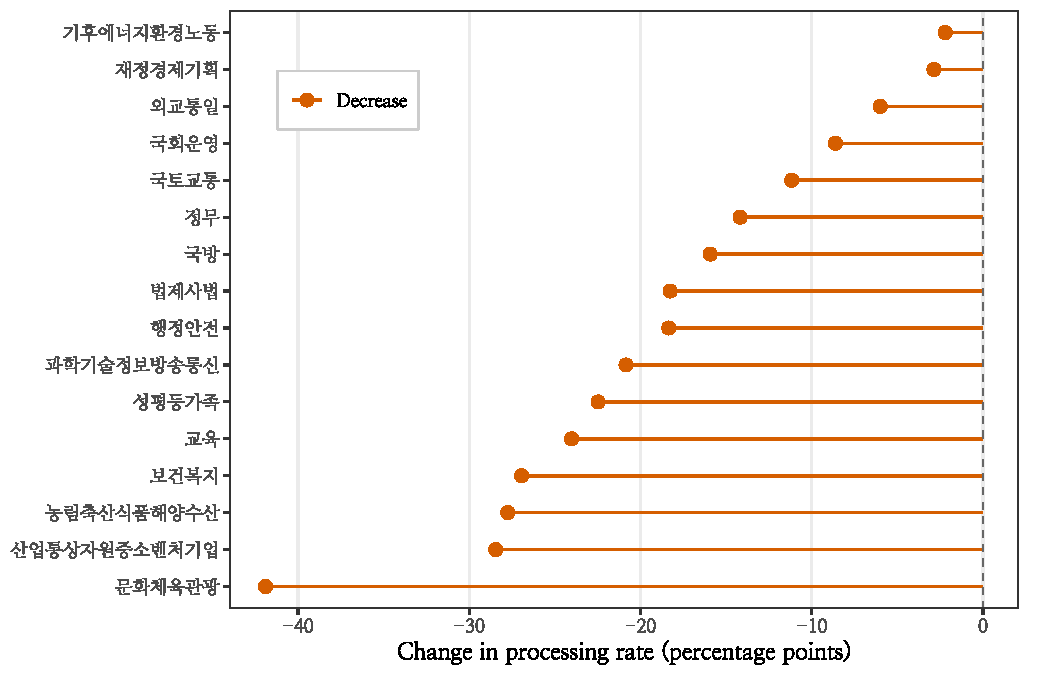
\includegraphics[width=\textwidth]{figures/art2_fig1_committee_crisis.pdf}
\caption{Committee-Level Changes in Bill Passage Rates Around December 3, 2024}
\label{fig:coef}
\end{figure}

Figure~\ref{fig:sc} visualizes the escalation of special counsel bill activity across assemblies, illustrating the growing claim on legislative processing capacity.

% R code for Figure 2 executed automatically (see figures/fig_2.R)

\begin{figure}[H]
\centering
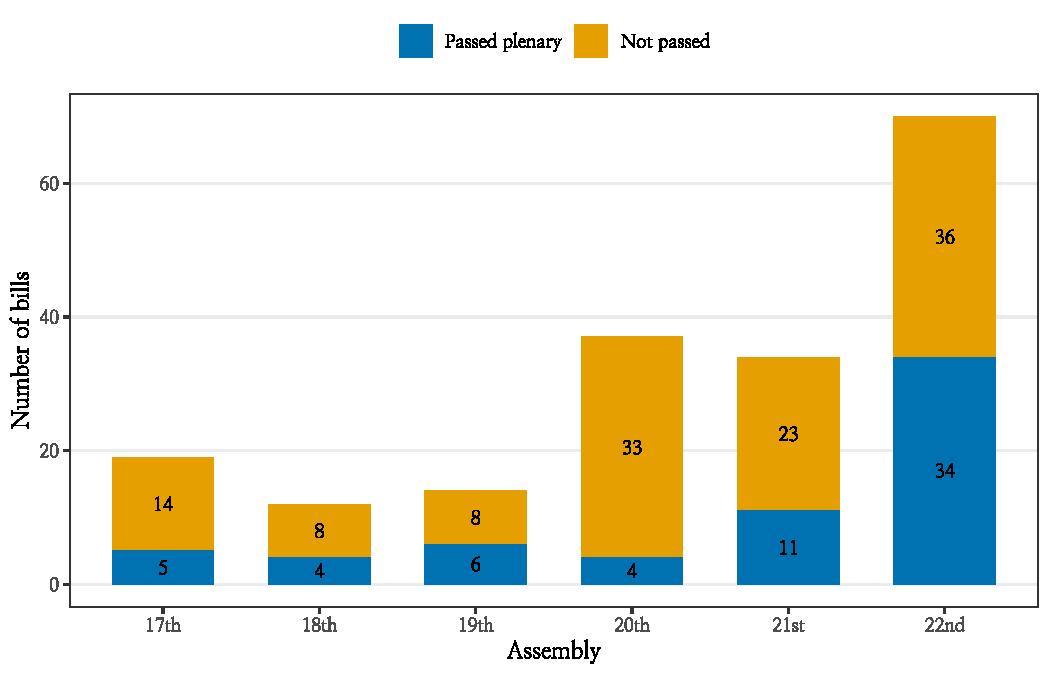
\includegraphics[width=\textwidth]{figures/art2_fig2_special_counsel_bills.pdf}
\caption{Special Counsel Bill Escalation Across National Assemblies}
\label{fig:sc}
\end{figure}

%% ============================================================
%%  5. DISCUSSION
%% ============================================================
\section{Discussion}

\subsection*{Three Mechanisms, One Interaction}

The results support a nuanced account of crisis-induced legislative displacement that cannot be captured by any single mechanism from the existing literature. I identify three distinct channels through which political crises affect routine legislation, each operating at a different institutional level.

The first mechanism is institutional capacity constraint, following \citet{baumgartner2009}. Legislative processing bandwidth is finite. Committee staff time, floor scheduling slots, and legislator attention are scarce resources, and accountability proceedings consume a disproportionate share during crises. This mechanism predicts a uniform decline across all non-crisis bill categories. The general legislative slowdown documented in Table~\ref{tab:main}, where all bill categories except political bills experienced reduced passage rates, is consistent with this baseline.

The second mechanism is strategic agenda reallocation, following \citet{cox2005} and \citet{petrocik1996}. The majority party deliberately redirects committee processing capacity to maximize electoral advantage during crisis periods. The bill processing speed gap (Table~\ref{tab:speed}), the 법사위 within-committee asymmetry (Table~\ref{tab:committee}), and the 기획재정위 anomaly all suggest selective rather than uniform displacement. Political bills are fast-tracked not merely because they are urgent but because accountability legislation serves the majority party's electoral goals. The finding that DPK sponsorship composition barely changed while processing rates collapsed confirms that the bottleneck operates downstream in committee scheduling, consistent with \citet{parkpy2026} and \citet{kimlee2026}.

The third mechanism is conditional shirking, following \citet{frank2021} and \citet{hoeyland2017}. Ruling-party legislators reduce floor participation when investigation-related political risk threatens their careers. The 20th Assembly evidence supports this mechanism: ruling-party absence increased substantially during the Park impeachment (Table~\ref{tab:absence}). But the 22nd Assembly evidence rejects it: PPP absence was unchanged. The conditionality is the key finding. Strategic shirking appears to be rational only when the ruling party holds sufficient seats for its absence to be consequential, a scope condition that the existing shirking literature has not identified.

The interaction between these mechanisms generates the double dissociation observed across the 20th and 22nd Assemblies (Table~\ref{tab:cross}). When the ruling party holds a near-majority, conditional shirking dominates, and ruling-party legislators withdraw from floor votes. But the opposition can sustain routine legislation through bipartisan cooperation, so livelihood bills are spared. When the opposition holds a supermajority, strategic reallocation dominates. The majority party monopolizes committee bandwidth for accountability legislation, and routine legislation collapses because the majority party faces no coalition constraint forcing it to maintain the routine agenda. Ruling-party shirking is irrelevant because the minority lacks the votes to affect outcomes regardless. This conditional model appears to be novel in the legislative studies literature and could not be derived from any single existing theoretical framework. The ``asymmetric constitutional hardball'' framework of \citet{fishkin2018} helps explain why: the serial reintroduction of special counsel bills consumes legislative bandwidth not as an unintended byproduct but as a form of institutional strategy whose costs are borne disproportionately by routine policy domains.

\subsection*{Comparison with Prior Work}

The finding that political crises crowd out routine legislation is consistent with \citet{pedrazzani2018}, who document a parallel pattern during Italy's economic crisis. However, the Korean case reveals three features that the Italian study does not capture. First, the displacement is asymmetric in a direction Pedrazzani and colleagues do not observe: political bills actually increase in passage probability. Second, the committee-level heterogeneity documented in Table~\ref{tab:committee}, ranging from a decline exceeding 40 percentage points for the Culture Committee to a substantial increase for the Strategy and Finance Committee, demonstrates that displacement is not uniform across institutional venues. Third, the cross-assembly comparison introduces a conditional element absent from the Italian analysis, where only a single legislature is examined.

The null result on co-sponsorship proximity is consistent with a conceptual limitation of the network proximity hypothesis when investigation targets are executive figures rather than legislators. \citet{katz2018} finds that Brazilian legislators distanced themselves from investigation targets who were fellow legislators embedded in coalition networks. In Korea, the targets (Yoon and Kim Kun-hee) are not members of the National Assembly, making co-sponsorship an inherently weak measure of political exposure. This suggests that network-based proximity measures may be appropriate for legislative corruption scandals but not for executive-branch crises, an important scope condition for future research.

The DPK's modest but statistically significant increase in absenteeism invites careful interpretation. On a base of approximately 13 percent, the 1.5 percentage-point increase represents a small relative change. With the DPK holding a supermajority, even a substantial attendance decline would rarely change bill outcomes. This finding may be better understood as a behavioral indicator of attention displacement, reflecting the cognitive burden of crisis governance, rather than as a causally consequential variable.

\subsection*{The Substantive Cost of Displacement}

The finding that political crises crowd out routine legislation risks being dismissed as tautological: when a president attempts an insurrection, of course the legislature drops everything to address it. The paper's contribution lies not in demonstrating that displacement occurs, which may indeed be intuitive, but in quantifying its magnitude, documenting its heterogeneity, and identifying the institutional mechanisms that transmit it. The decline in livelihood bill resolution documented in Table~\ref{tab:main} translates to concrete policy consequences. Healthcare reform bills, education funding measures, pension adjustments, and consumer protection legislation that would have advanced under normal conditions stalled in committee while 법사위 processed its eighth iteration of a special counsel bill. The hearing data reinforce this picture: post-insurrection hearings were not only far less frequent (70 versus 503) but also involved fewer speeches per session and fewer participating legislators. The entire legislative apparatus contracted, concentrating its diminished capacity on a narrow band of accountability-related proceedings.

The 기획재정위 anomaly sharpens the substantive implications. The fact that fiscal legislation was exempted from the general freeze (Table~\ref{tab:committee}) demonstrates that the displacement is not merely a function of reduced capacity but reflects choices about which policy domains are ``essential'' during crisis governance. Both parties appear to have recognized that economic disruption carries immediate electoral costs, creating a bipartisan floor for fiscal legislation that does not extend to healthcare, education, or welfare bills. This selective exemption suggests that the cost of accountability falls disproportionately on policy domains whose beneficiaries have less immediate political leverage, a distributional consequence with normative implications for democratic representation.

\subsection*{Limitations}

Several limitations constrain the conclusions I can draw from this analysis. First, the December 3 insurrection is not a ``typical'' political crisis. Any findings may be specific to this extraordinary event and ungeneralizable to routine special counsel proceedings. The cross-assembly comparison helps but provides only two cases under different structural conditions, which is insufficient for a general theory. A stacked event-study design exploiting all seven Korean special counsel investigations since 1999 would strengthen identification but requires constructing committee-level data for earlier assemblies where records may be incomplete.

Second, the seasonal confound remains a concern. The December 3 event occurred during the normal end-of-session wind-down, and disentangling crisis effects from seasonal patterns requires formal seasonal adjustment or a within-month comparison using daily meeting timestamps. While the magnitude of the observed decline far exceeds normal seasonal variation, and the January 2025 trough is substantially below the January 2026 level, I cannot fully rule out seasonal contamination with the current design.

Third, the bill classification is coarse. Keyword matching captures only obvious markers, and some bills may be misclassified. A refined classification using the 60,925 propose-reason texts available in the KNA database would sharpen the categorization, though the direction and magnitude of the documented asymmetry suggest the qualitative pattern is robust to classification refinement.

Fourth, roll-call votes capture floor participation but not committee participation, which is the more direct measure of the governance vacuum. Committee meeting records track which bills were discussed but not which legislators were present. Hearing speech frequency provides a behavioral proxy but not a direct attendance measure. Future work with more granular committee attendance data could directly test whether investigation-period committee absenteeism varies by proximity to targets.

Fifth, the 22nd Assembly is ongoing. Post-December 3 bills have had less time to be processed, creating a mechanical time-to-maturation confound. As discussed in Section 3, survival models with right-censoring and restricted comparison windows offer concrete paths to address this concern. The processing speed evidence (Table~\ref{tab:speed}), showing that the gap between political and livelihood bill processing widened post-crisis, suggests that the asymmetry is not merely a function of time, but the completed assemblies in a stacked design would eliminate this concern entirely.

%% ============================================================
%%  6. CONCLUSION
%% ============================================================
\section{Conclusion}

This paper documents a previously unexamined trade-off in democratic governance: the pursuit of executive accountability through legislative mechanisms appears to impose substantial collateral costs on routine legislation. Using the December 3, 2024 insurrection in South Korea as a natural experiment, I find that livelihood bill resolution rates declined substantially, with an additional penalty beyond the general legislative slowdown (Table~\ref{tab:reg}, column 3: $\beta_3 = -0.059$, SE $= 0.020$, $p < 0.01$). Political bills, by contrast, were fast-tracked through the committee system, receiving action in a fraction of the time required for routine legislation (Table~\ref{tab:speed}).

The contribution is threefold. First, the attention displacement finding extends the agenda-setting capacity literature \citep{baumgartner2009, boydstun2014} from gradual, cross-national agenda shifts to within-legislature dynamics around sharp political discontinuities. Second, the conditional shirking result, ruling-party absence increases during crises only when the party holds sufficient seats for absence to matter, identifies a scope condition that the legislative shirking literature \citep{frank2021, gavoille2017} has not previously documented. Third, the double dissociation across the 20th and 22nd Assemblies suggests that crisis-induced legislative damage operates through substitutable channels conditioned by institutional structure, a theoretical insight that unifies the capacity constraint, strategic reallocation, and conditional shirking mechanisms.

These findings carry implications for institutional design. If legislative processing capacity is indeed zero-sum, constitutional arrangements that separate accountability proceedings from routine legislation, such as dedicated investigation committees or parallel processing tracks, could reduce the collateral damage documented here. The Korean National Assembly's proportional committee chair allocation, which differs from the American majority-party-controls-all model \citep{cox2005}, creates distinctive dynamics that comparative legislative scholars may wish to examine in other proportional-representation systems.

Future research should pursue three directions. First, a stacked event-study design exploiting multiple special counsel investigations across the 19th through 22nd Assemblies would test whether the attention displacement mechanism generalizes beyond the December 3 case. Second, refined bill classification using natural language processing on propose-reason texts could sharpen the measurement of ``livelihood'' and ``political'' categories. Third, comparative analysis with Brazil's Lava Jato experience \citep{katz2018} and Italy's economic crisis \citep{pedrazzani2018} could test whether the conditional model holds across different institutional settings. The cost of accountability is a topic that deserves systematic attention from scholars of democratic governance.

\noindent\textit{This working paper was generated by AI research agents as an
experimental output. It has not been peer-reviewed or fact-checked.
Do not cite or use in any academic, policy, or professional context.}

\bibliographystyle{apsr}
\bibliography{references_r4}

\end{document}
